\documentclass[10pt]{article}

\usepackage{araim-common}
\usepackage{araim-tex}

\makeatletter
\def\blfootnote{\xdef\@thefnmark{}\@footnotetext}
\makeatother

\title{Questions about Prediction in STCOS Model}
%\date{}
\author{Andrew M. Raim
\vspace{0.5em} \\
Center for Statistical Research and Methodology, U.S. Census Bureau
}

\begin{document}

\maketitle

% ---------------------------------------------------
\section{Introduction}
\label{sec:intro}
Recall that the process model in \citet{BradleyEtAl2016-STAT} is
%
\begin{align*}
Y_t^{(\ell)}(A) = h(A)^T \mu_B + \psi_t^{(\ell)}(A)^T \eta + \xi_t^{(\ell)}(A).
\end{align*}
%
Our first objectives are to reproduce Figures 1(g) and 1(h). These represent 2013 3-year ACS estimates and standard deviations from the model. The model-based estimate from the paper is written as
%
\begin{align*}
\hat{Y}_t^{(\ell)}(A) = \E[ Y_t^{(\ell)}(A) \mid \{ Z_t^{(\ell)}(A) \} ],
\quad A \in D_{t,A}^{(\ell)};
\quad t = T_L, \ldots, T_U, 
\quad \ell = 1,3,5.
\end{align*}
%
From this expression, the quantity $\hat{Y}_t^{(\ell)}(A)$ could be approximated using MCMC draws $\{ Y_t^{(\ell, r)}(A) : r = 1, \ldots, R \}$ as
%
\begin{align*}
\frac{1}{R} \sum_{r=1}^R Y_t^{(\ell, r)}(A).
\end{align*}
%
However, this does not permit predictions for parts of space-time that did not have observations, which is what is needed to reproduce Figures 1(g) and 1(h). Then how should we compute predictions? Another idea is to use draws of the parameters $\{ \eta^{(r)} : r = 1, \ldots, R \}$ and $\{ \mu_B^{(r)} : r = 1, \ldots, R \}$, so that
%
\begin{align}
\hat{Y}_t^{(\ell)}(A) \approx \frac{1}{R} \sum_{r=1}^R \mu_t^{(\ell, r)}(A), \quad
\text{where $\mu_t^{(\ell, r)}(A) = h(A)^T \mu_B^{(r)} + \psi_t^{(\ell)}(A)^T \eta^{(r)}$}.
\label{eqn:predict-mcmc}
\end{align}
%
To compute the posterior standard deviation, I am guessing that the computation
\begin{align*}
\sigma_t^{(\ell)}(A) \approx \left[
\frac{1}{R-1} \sum_{r=1}^R \left\{ \mu_t^{(\ell, r)}(A) - \overline{\mu_t^{(\ell, \cdot)}(A)} \right\}^2
\right]^{1/2}, \quad
\text{where $\overline{\mu_t^{(\ell, \cdot)}(A)} = \frac{1}{R} \sum_{r=1}^R \mu_t^{(\ell, r)}(A)$}
\end{align*}
%
was used.

A complication here is that we need to compute $\psi_t^{(\ell)}(A)$ for the new space-time point, which is also not quite clear. The following block of Matlab code in \code{data\_organization.m} computes the basis functions.

\begin{lstlisting}
%Basis Functions
SGBF1 = ArealBi2_spacetime(county1,2013,level,[],[],100,0.5,0.5);
SGBF3 = ArealBi2_spacetime(county3,2009:2013,level,[],[],100,0.5,0.5);
SGBF1_2012 = ArealBi2_spacetime(county1_2012,2012,level,[],[],100,0.5,0.5);
SGBF2_2012 = ArealBi2_spacetime(county2_2012,2010:2012,level,[],[],100,0.5,0.5);
SGBF3_2012 = ArealBi2_spacetime(county3_2012,2008:2012,level,[],[],100,0.5,0.5);
SGBF1_2011 = ArealBi2_spacetime(county1_2011,2011,level,[],[],100,0.5,0.5);
SGBF2_2011 = ArealBi2_spacetime(county2_2011,2009:2011,level,[],[],100,0.5,0.5);
SGBF3_2011 = ArealBi2_spacetime(county3_2011,2007:2011,level,[],[],100,0.5,0.5);
SGBF1_2010 = ArealBi2_spacetime(county1_2010,2010,level,[],[],100,0.5,0.5);
SGBF2_2010 = ArealBi2_spacetime(county2_2010,2008:2010,level,[],[],100,0.5,0.5);
SGBF3_2010 = ArealBi2_spacetime(county3_2010,2006:2010,level,[],[],100,0.5,0.5);
SGBF1_2009 = ArealBi2_spacetime(county1_2009,2009,level,[],[],100,0.5,0.5);
SGBF2_2009 = ArealBi2_spacetime(county2_2009,2007:2009,level,[],[],100,0.5,0.5);
SGBF3_2009 = ArealBi2_spacetime(county3_2009,2005:2009,level,[],[],100,0.5,0.5);
SGBF1_2008 = ArealBi2_spacetime(county1_2008,2008,level,[],[],100,0.5,0.5);
SGBF2_2008 = ArealBi2_spacetime(county2_2008,2006:2008,level,[],[],100,0.5,0.5);
SGBF1_2007 = ArealBi2_spacetime(county1_2007,2007,level,[],[],100,0.5,0.5);
SGBF2_2007 = ArealBi2_spacetime(county2_2007,2005:2007,level,[],[],100,0.5,0.5);
SGBF1_2006 = ArealBi2_spacetime(county1_2006,2006,level,[],[],100,0.5,0.5);


S = cat(1,SGBF1,SGBF1_2012,SGBF1_2011,SGBF1_2010,SGBF1_2009,SGBF1_2008,SGBF1_2007,SGBF1_2006,...
    SGBF2_2012,SGBF2_2011,SGBF2_2010,SGBF2_2009,SGBF2_2008,SGBF2_2007,...
    SGBF3,SGBF3_2012,SGBF3_2011,SGBF3_2010,SGBF3_2009);

[S1,idx]=licols(S);
\end{lstlisting}
%
The matrix \code{S1} was used as the design matrix in the MCMC. One issue is that licols does not appear to be a built-in Matlab function. I found a version on the web at \url{https://www.mathworks.com/matlabcentral/answers/49984-how-to-remove-dependent-rows-in-a-matrix}, but am not sure if this is the same thing Jon used. But let's move forward assuming that it is. To set up the covariate for 3-year 2013 ACS, I assume I should run something like this,
%
\begin{lstlisting}
SGBF3 = ArealBi2_spacetime(county3, 2013, level, [], [], 100, 0.5, 0.5);
[SGBF3_1, idx] = licols(SGBF3);
\end{lstlisting}
%
Here, I am attempting to compute basis functions for 2013 on the complete set of counties, which are contained in \code{county3}. I am then using \code{idx} to pick out the columns of \code{SGBF3} corresponding to the ones used to fit the MCMC. Now, \code{SGBF3\_1} is a $3109 \times 1250$ matrix. We also need to compute the overlaps $h(A)$ that correspond to this area. The matrix \code{H.new} of these overlaps should be  $3109 \times 3109$; I am thinking this should just be the identity matrix, since predictions are being requested on the fine-level spatial support (denoted $D_B$ in the paper).

\vspace{0.5em}
\noindent
To summarize, the outstanding questions were:
%
\begin{enumerate*}
\item How did Jon compute predictions and their standard deviations?
\item Which \code{licols} function did Jon use?
\item How did Jon compute the design matrix $S$ and the overlap matrix $H$ for the 3-year 2013 ACS domain, if they are needed?
\end{enumerate*}
%
Using the assumptions I have made above, I get the results in Figure~\ref{fig:post}, which appear to be somewhat close to Figures 1(g) and 1(h) in \citet{BradleyEtAl2016-STAT}. Note that I am using only 1,000 of the available 10,000 draws because I am using my home PC which has limited memory.

\begin{figure}
\centering
\begin{subfigure}[b]{.95\textwidth}
  \centering
  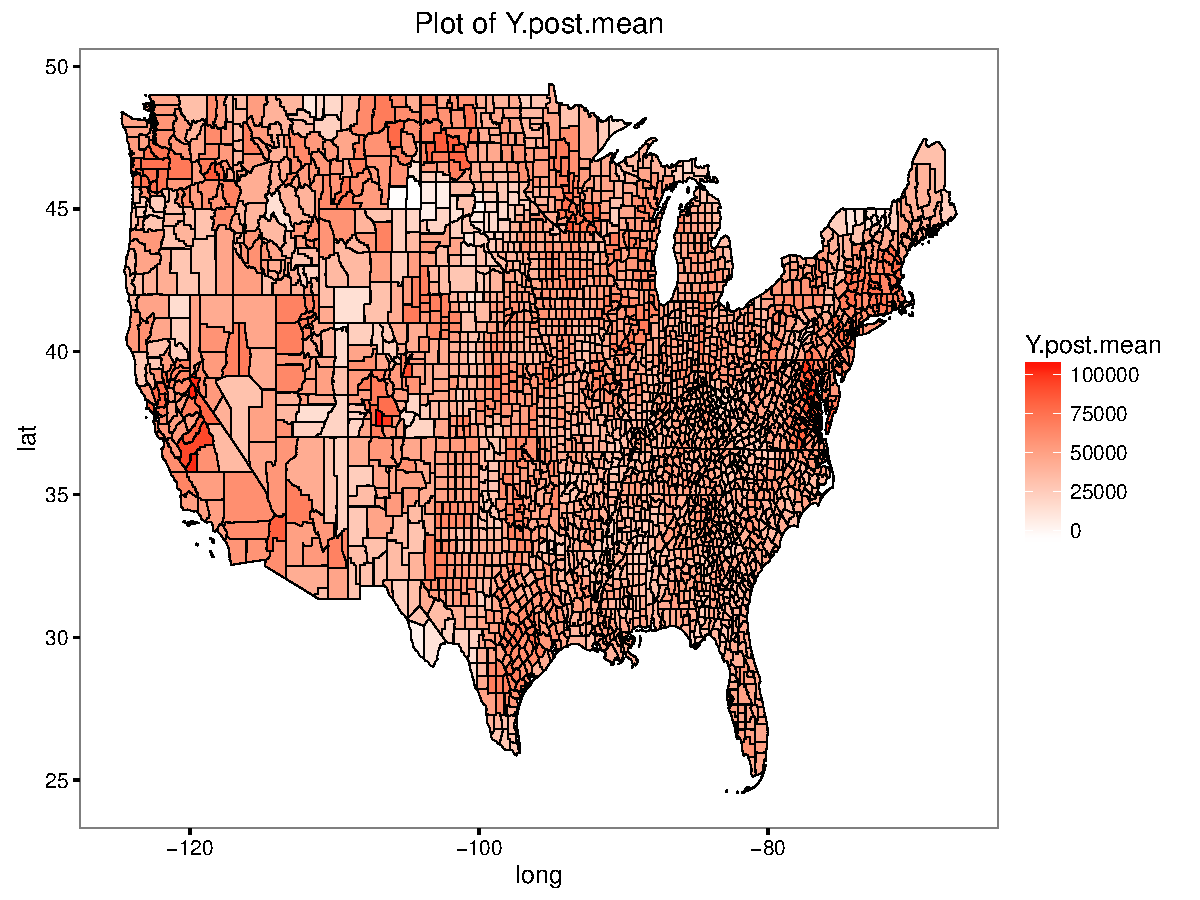
\includegraphics[width=0.95\textwidth]{figures/post-mean.pdf}
  \label{fig:post-mean}
\end{subfigure}

\begin{subfigure}[b]{.95\textwidth}
  \centering
  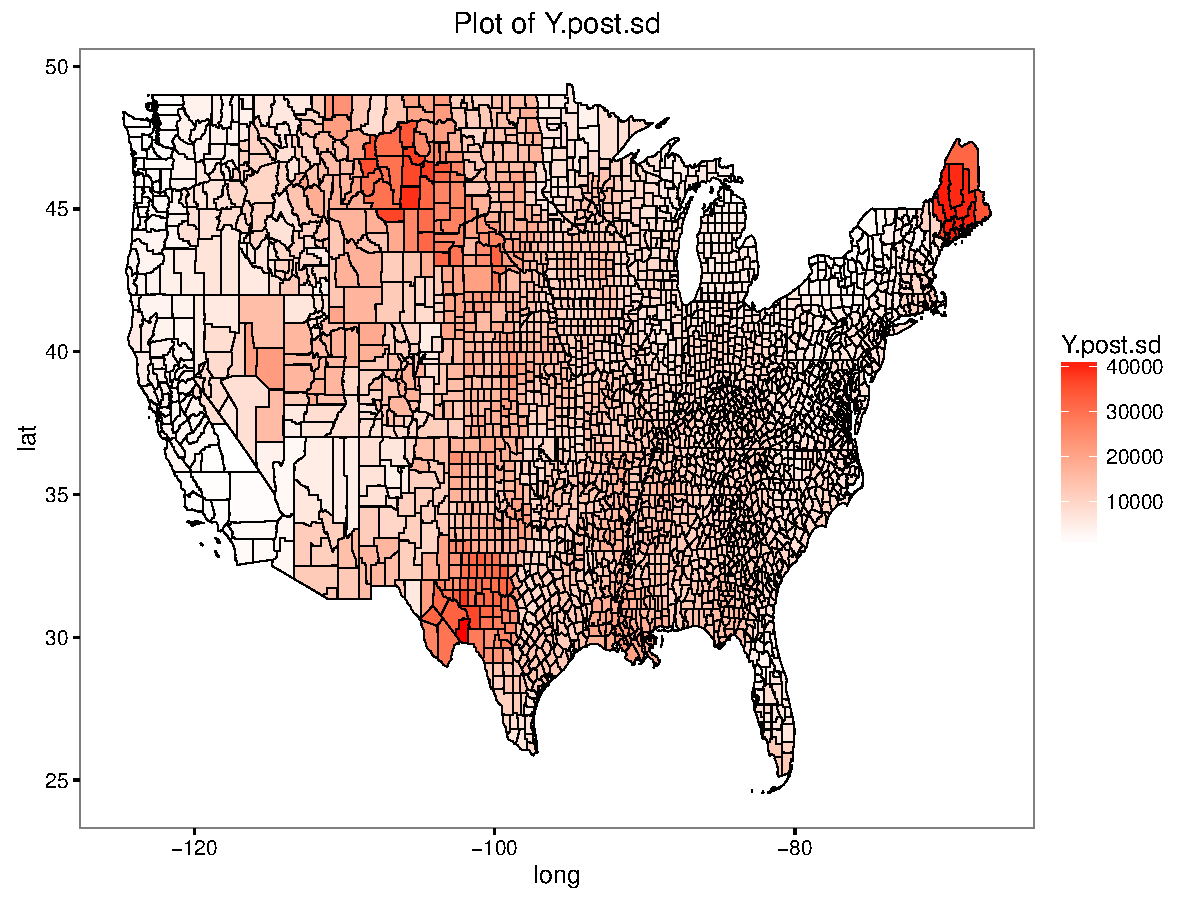
\includegraphics[width=0.95\textwidth]{figures/post-sd.pdf}
  \label{fig:post-sd}
\end{subfigure}
\caption{Posterior mean and standard deviation using my assumptions.}
\label{fig:post}
\end{figure}

We were having some questions about diagnostics. Figures~\ref{fig:diag-mu}
through~\ref{fig:diag-sig2K} show
trace plots and histograms for draws obtained from the draws used to produce
Figure~\ref{fig:post} (which have the alleged ``mistake'' in the $\mu_B$ step
where the latest $\sigma_\xi^2$ value is not used). The draws for $\mu_B$,
$\eta$, $\xi$, $\sigma_\mu^2$, and $\sigma_K^2$ show good mixing. Jon's code
does not include the $\sigma_\xi^2$ step, so a plot corresponding to this
variable is not shown.

\begin{figure}
\centering
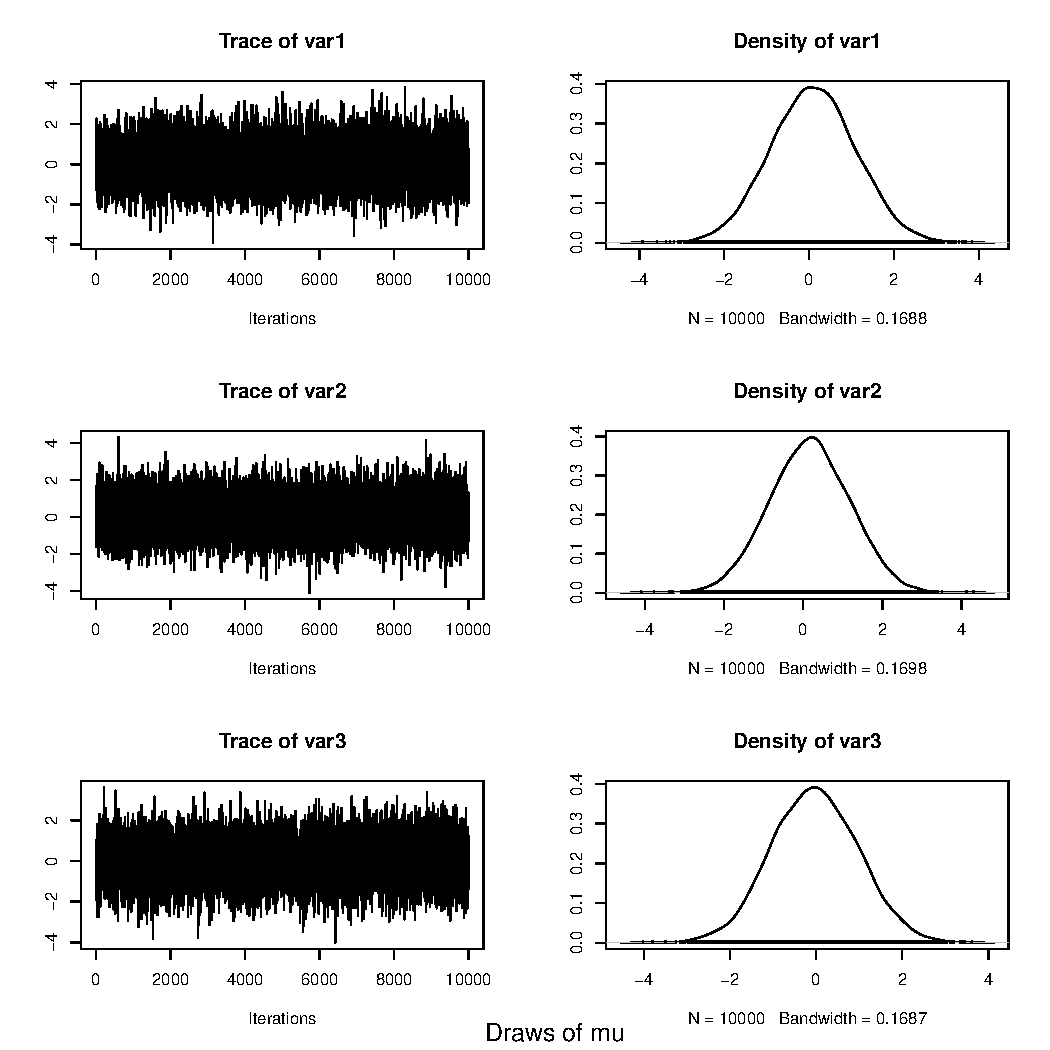
\includegraphics[width=0.95\textwidth]{figures/diag-mu.pdf}
\caption{}
\label{fig:diag-mu}
\end{figure}

\begin{figure}
\centering
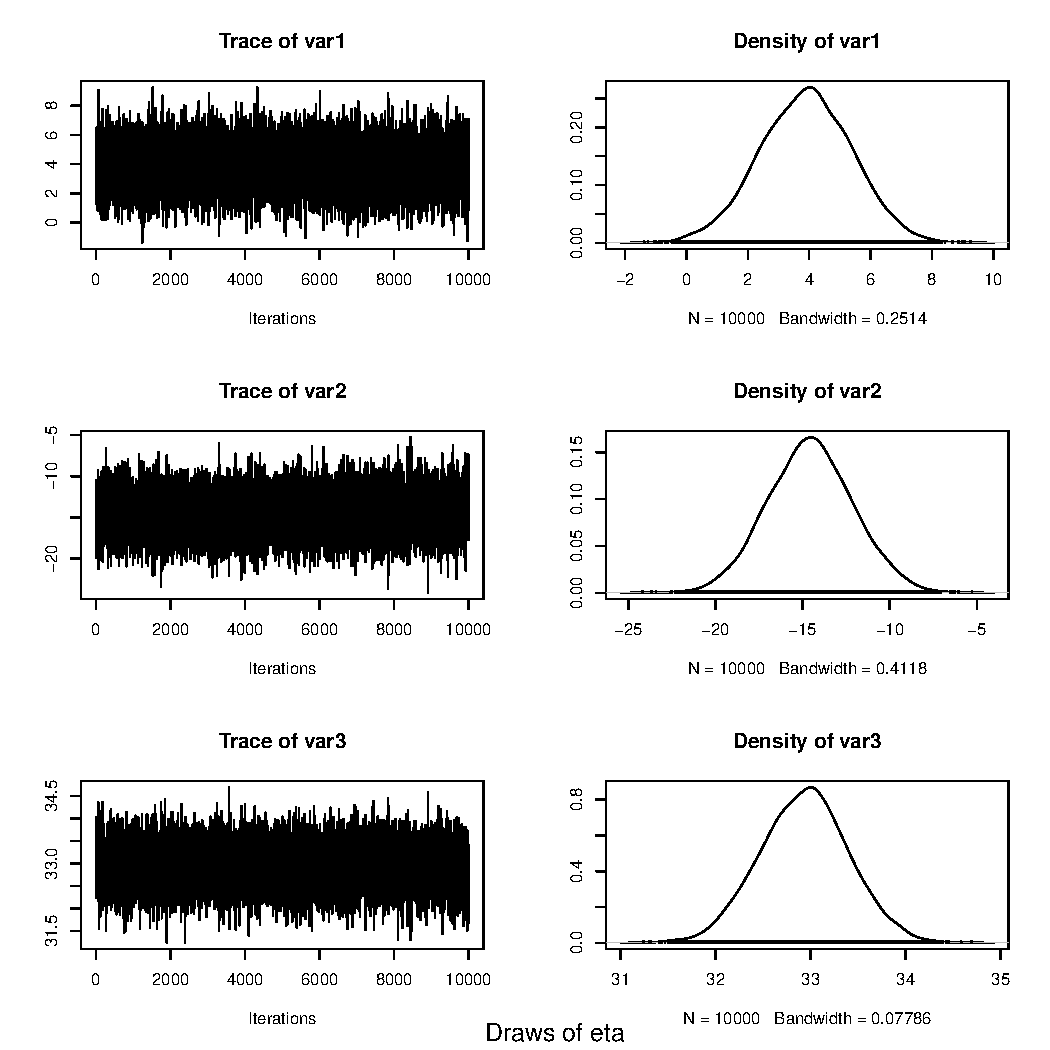
\includegraphics[width=0.95\textwidth]{figures/diag-eta.pdf}
\caption{}
\label{fig:diag-eta}
\end{figure}

\begin{figure}
\centering
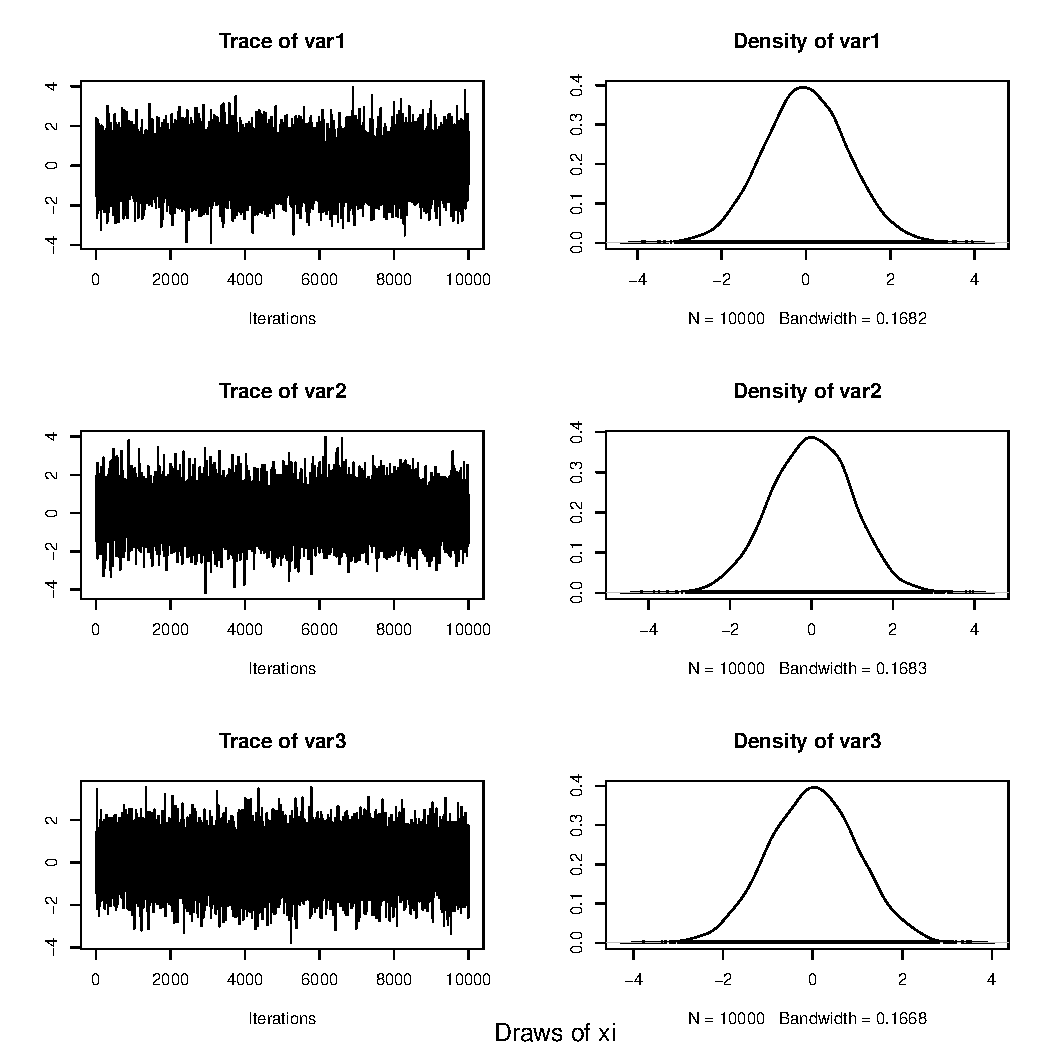
\includegraphics[width=0.95\textwidth]{figures/diag-xi.pdf}
\caption{}
\label{fig:diag-xi}
\end{figure}

\begin{figure}
\centering
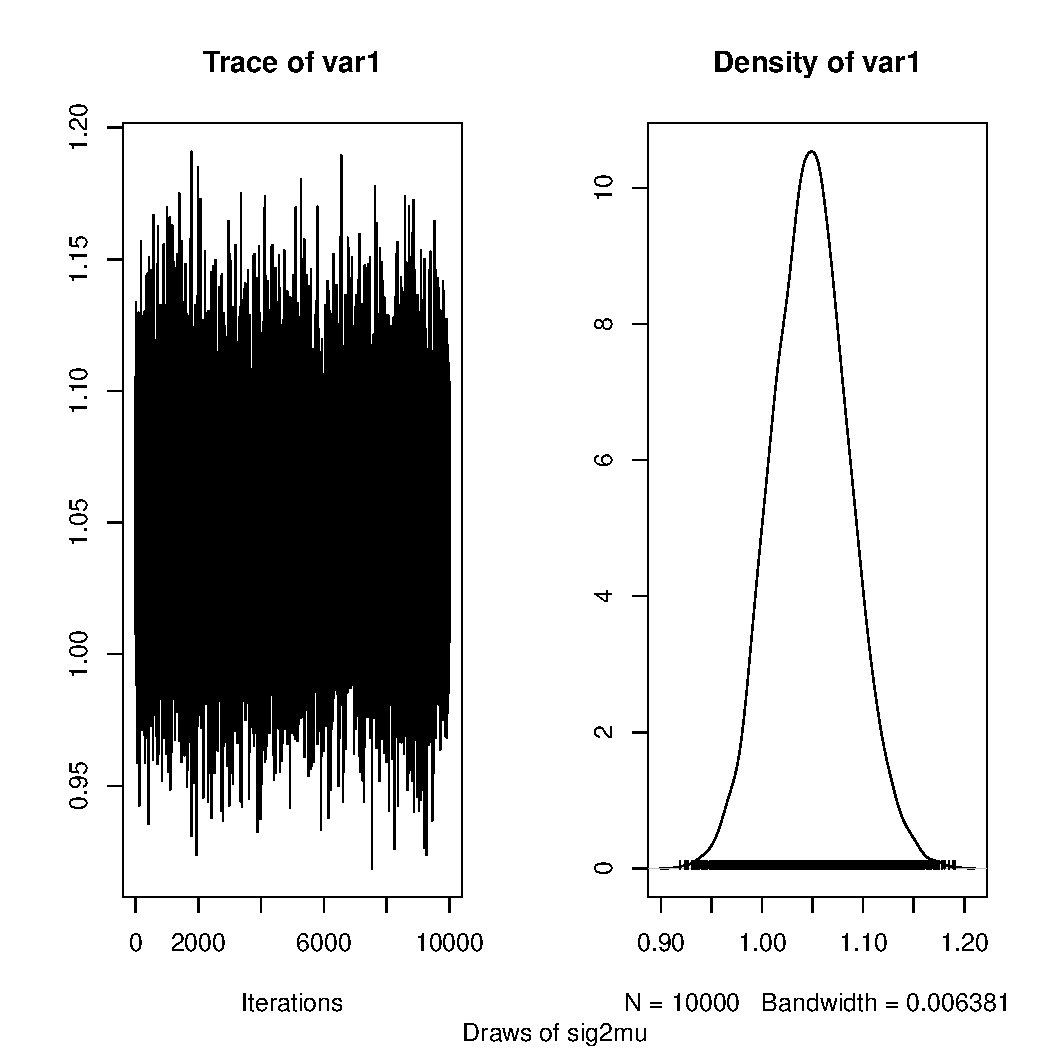
\includegraphics[width=0.95\textwidth]{figures/diag-sig2mu.pdf}
\caption{}
\label{fig:diag-sig2mu}
\end{figure}

\begin{figure}
\centering
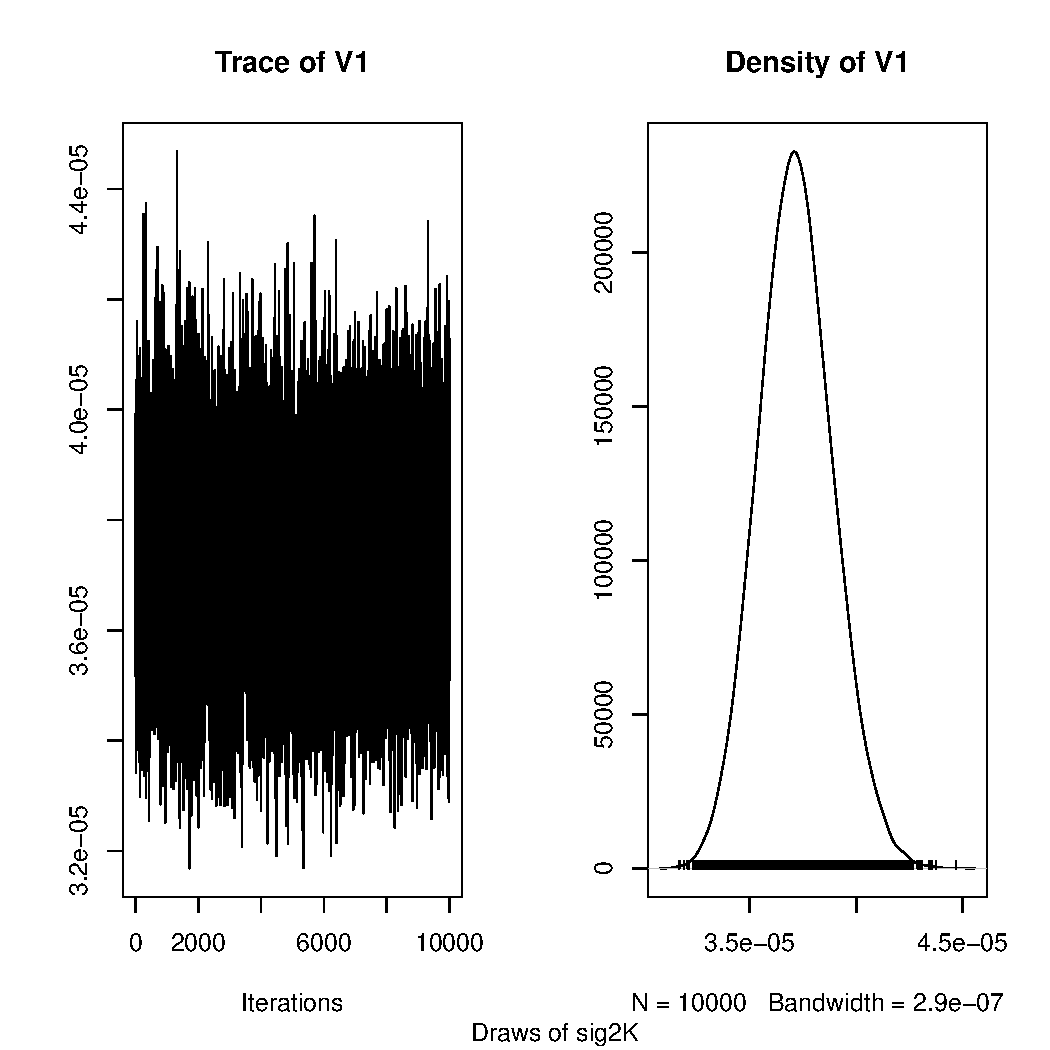
\includegraphics[width=0.95\textwidth]{figures/diag-sig2K.pdf}
\caption{}
\label{fig:diag-sig2K}
\end{figure}

\bibliographystyle{plainnat}
\bibliography{references}
%\input{references.bbl}

\end{document}
